\documentclass[12pt]{article}
\usepackage{amsfonts}
\usepackage{amsmath}
\usepackage{graphicx}
\usepackage{xcolor}
\newcommand{\blue}[1]{\textcolor{blue}{#1}}
\usepackage{float}
\usepackage[caption = false]{subfig}
\usepackage{/Users/timbarry/optionFiles/mymacros}
\DeclareMathOperator*{\argmin}{arg\,min}

\begin{document}
\noindent
Tim, Gene, Kathryn
\begin{center}
\textbf{CRISPR genome editing, single-cell sequencing, and exponential family measurement error models}
\end{center}

\begin{abstract}
CRISPR genome engineering and single-cell sequencing have transformed biological discovery. Single-cell CRISPR screens unite these two technologies, linking genetic perturbations in individual cells to changes in gene expression and illuminating regulatory networks underlying diseases. In this work we study single-cell CRISPR screens from a statistical perspective. First, we demonstrate on real data that a standard method for estimation and inference in single-cell CRISPR screens — “thresholded regression” — exhibits attenuation bias and a bias-variance tradeoff as a function of an intrinsic tuning parameter. We recover these phenomena in precise theoretical terms in an idealized Gaussian setting. Next, we introduce GLM-EIV (“generalized linear model with errors-in-variables”), a new method for single-cell CRISPR screen analysis. GLM-EIV generalizes the classical errors-in-variables model to response distributions and sources of measurement error that are exponential family-distributed, overcoming limitations of thresholded regression. We develop a computational infrastructure to deploy GLM-EIV across hundreds or thousands of processors on clouds (e.g., Microsoft Azure) and high-performance clusters. Leveraging this infrastructure, we apply GLM-EIV to analyze two recent, large-scale, single-cell CRISPR screen datasets, yielding new biological insights.
\end{abstract}

\section{Introduction}
CRISPR is a genome engineering tool that has enabled scientists to precisely edit human and nonhuman genomes, opening the door to new medical therapies \cite{Rothgangl2021,Musunuru2021} and transforming basic biology research \cite{Przybyla2021}. Recently, scientists have paired CRISPR genome engineering with single-cell sequencing \cite{Dixit2016,Datlinger2017}. The resulting assays, known as a ``single-cell CRISPR screens,'' link genetic perturbations in individual cells to changes in gene expression, illuminating regulatory networks underlying human diseases and other traits \cite{Morris2021a}.

Despite their promise, single-cell CRISPR screens present substantial statistical challenges. A major difficulty is that CRISPR perturbations are unobservable and assigned stochastically to cells. As a consequence, one cannot know with certainty which cells were perturbed. Instead, one must leverage an indirect, noisy proxy of perturbation presence or absence -- namely, transcribed barcode counts -- to ``guess'' which cells were perturbed. Using these imputed perturbation assignments, one can attempt to estimate the effect of the perturbation on gene expression. The standard approach, which we call ``thresholded regression'' or the ``thresholding method,'' is to assign perturbation identities to cells by simply thresholding the barcode counts.

We study estimation and inference in single-cell CRISPR screens from a statistical perspective, formulating the data generating mechanism using a new class of errors-in-variables (or measurement error) models. We assume that the response variable $y$ is a GLM of an underlying predictor variable $x^*$. We do not observe $x^*$ directly; rather, we observe a noisy version $x$ of $x^*$ that itself is a GLM of $x^*$. The goal of the analysis is to estimate the effect of $x^*$ on $y$ using the observed data $(x , y)$ only. In the context of the biological application, $x^*$, $y$, and $x$ are CRISPR perturbations, gene expressions, and barcode counts, respectively.

Our work makes two main contributions. First, we study the thresholding method from empirical and theoretical perspectives. Notably, we demonstrate on real data that the thresholding method exhibits attenuation bias and a bias-variance tradeoff as a function of the selected threshold, and we recover these phenomena in precise mathematical terms in an idealized Gaussian model. Second, we introduce a new method for estimation and inference in single-cell CRISPR screens that accounts for the measurement error inherent in the experiment. The method, called \textit{GLM-EIV} (generalized linear model with errors-in-variables), implicitly estimates the probability that each cell was perturbed, obviating the need to explicitly impute perturbation assignments via thresholding or another heuristic. Theoretical analyses and simulation studies indicate that GLM-EIV outperforms the thresholding method in large regions of the parameter space.

We implement several statistical accelerations (that likely are of independent utility) to bring the cost of GLM-EIV down to within an order of magnitude of the thresholding method. Finally, we develop a computational infrastructure to deploy GLM-EIV at-scale across hundreds or thousands of processors on clouds (e.g., Microsoft Azure) and high-performance clusters. Leveraging this infrastructure, we apply GLM-EIV to analyze two recent, large-scale, high multiplicity-of-infection single-cell CRISPR screen datasets, yielding new biological and statistical insights. 

\section{Background and analysis challenges}

Our focus in this work is on high multiplicity-of-infection (MOI), enhancer-targeting, single-cell CRISPR screens. In this section we cover relevant biological background and motivation.
\\ \\
\textbf{P1}: The human genome consists of genes (segments of DNA that code for proteins), enhancers (segments of DNA that regulate the expression of one or more genes), and other genomic regions. Genome-wide association studies have revealed that the majority ($>95\%$) of variants associated with diseases lie outside genes and (very likely) inside enhancers. These noncoding variants contribute to disease by modulating the expression one or more genes, which in turn encode proteins that affect the phenotype. A central open challenge in genetics, therefore, is to link enhancers that harbor disease-associated variants to the genes that they target at genome-wide scale.
\\ \\
\textbf{P2}: High MOI single-cell CRISPR screens are the most promising biotechnology for solving this problem. \blue{Describe the experimental protocol here. Explain that we use the terms ``barcodes'' and ``gRNAs'' interchangeably, as polyadenylated gRNAs serve as barcodes in CROP-seq. Link to Figure \ref{analysis_challenges}.}
\\ \\
\textbf{P3}: Single-cell CRISPR screens pose several core analysis challenges. \blue{Describe the analysis challenges here: (i) unobserved perturbation; (ii) existence of background reads; (iii) highly discrete count data; (iv) nuisance variables}.

\begin{figure}[h!]
	\centering
	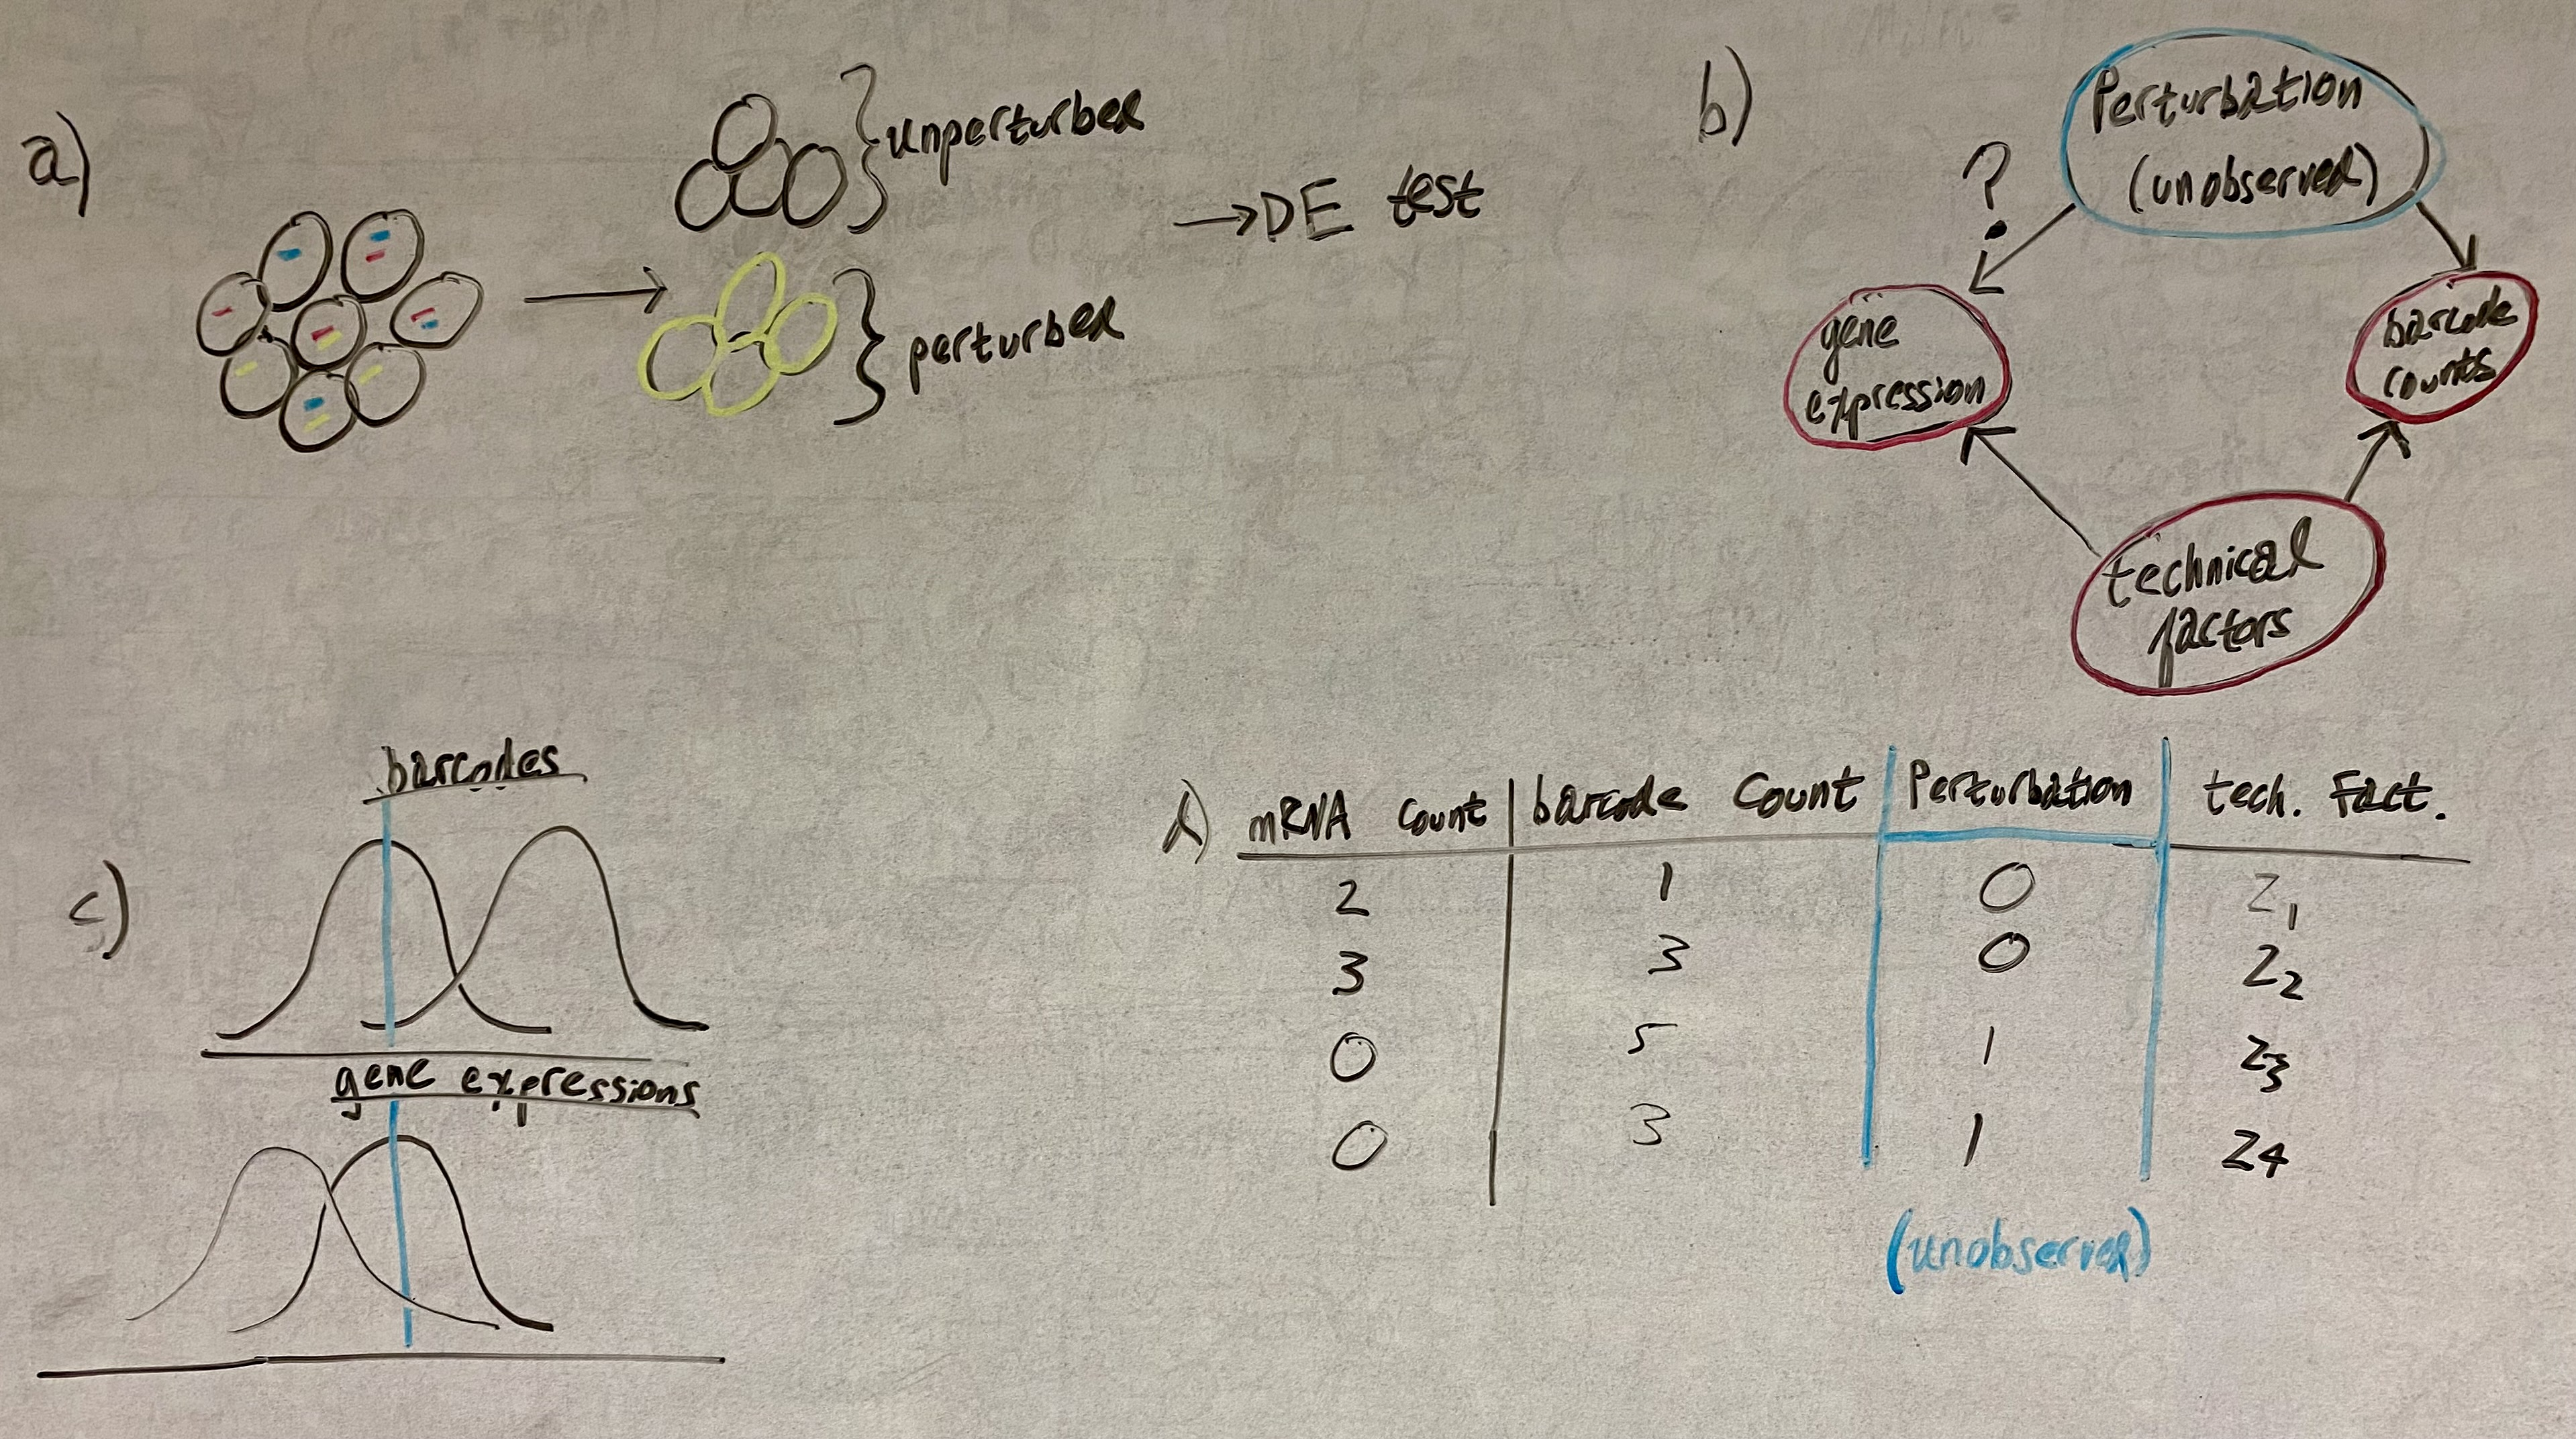
\includegraphics[width=0.9\linewidth]{analysis_challenges}
	\caption{\textbf{Overview of experimental design and analysis challenges}: \textbf{a,} Experimental design. For a given perturbation (e.g., the perturbation represented in yellow), we partition the cells into two groups: those that received the perturbation, and those that did not receive the perturbation. For a given gene, we conduct a differential expression analysis across the two groups of cells, yielding an estimate of the impact of the given perturbation on the given gene. \textbf{b,} DAG representing the variables in the analysis. The perturbation (unobserved) affects both gene expression and gRNA expression; technical factors (e.g., batch, sequencing depth, etc.) act as nuisance variables. The target of inference is the effect of the perturbation on gene expression (denoted with question mark). \textbf{c,} Schematic illustrating ``background reads.'' The gRNA modality has a nonzero, ``background read'' distribution even in the absence of a perturbation, complicating the assignment of perturbations to cells. \textbf{d}, Example data for a given perturbation-gene pair. Notice that (i) the perturbations are unobserved, and (ii) the gene and gRNA expression data take the form of discrete counts.}
	\label{analysis_challenges}
\end{figure}

\section{Related work}

Motivated by the challenges of single-cell data, several authors recently have extended statistical models that (implicitly or explicitly) assume Gaussianity and homoscedasticity to a broader class of exponential family distributions. For example, Lin, Lei, and Roeder \cite{Lin2021} developed eSVD, an extension of SVD to exponential family and curved Gaussian responses. Unlike SVD, eSVD models the relationship between the mean and variance of a gene's expression level, a phenomenon induced by the countedness of single-cell data \cite{Lause2021}.
Similarly, Townes et al.\ \cite{Townes2019} proposed GLM-PCA, an extension of PCA that directly models Poisson- or negative binomially-distributed gene expression counts. We see our work as a continuation of this broad effort to ``port'' common statistical methods and models to single-cell count data. Our focus, however, is on regression rather than dimension reduction: we extend the classical errors-in-variables model to response distributions and sources of measurement error that are exponential family-distributed.

The closest parallels to our work in the statistical methodology literature are Gr\"{u}n \& Leisch \cite{Grun2008} and Ibrahim \cite{Ibrahim1990}. Gr\"{u}n \& Leisch considered estimation and inference in a $k$-component mixture of GLMs. While we prefer to view the GLM-EIV model as an errors-in-variables model,  the GLM-EIV model is equivalent to a two-component mixture of \textit{products} of GLM densities. Ibrahim derived a method for fitting GLMs in the presence of missing-at-random covariates. Our method, by contrast, involves fitting two conditionally independent GLMs in the presence of a totally latent covariate. Thus, while Ibrahim is a helpful reference, our estimation and inference tasks are more complex.

The genomics literature has produced several applied methods for linking perturbations to changes in gene expression in single-cell CRISPR screens: SCEPTRE \cite{Barry2020}, MIMOSCA \cite{Dixit2016}, and scMAGeCK \cite{Yang2019}. These methods in general are focused on hypothesis testing rather than estimation; none, for instance, produces a confidence interval for the effect size of a perturbation on gene expression change. Additionally, two of these methods (MIMOSCA and scMAGeCK) use (possibly penalized) linear models to model gene expressions, thereby disregarding the countedness and sparsity of the data. 

\section{Thresholding method}

In this section we study the thresholding method from empirical and theoretical perspectives. First, we define some notation.

\blue{Let $n \approx 100,000 - 250,000$ be the number of cells in the experiment. Consider a single perturbation-gene pair. For cell $i \in \{ 1, \dots, n \},$ let $p_i \in \{ 0,1 \}$ indicate whether the cell was perturbed, $m_i \in \N$ be the number of observed gene UMIs, $g_i \in \N$ be the number of observed gRNA UMIs, $l^m_i \in \N$ be the gene library size, and $z_i \in \R^{d-1}$ be a vector of technical factors (e.g., batch, percent mitochondrial reads, etc.). The thresholding method is defined as follows:}
\blue{
\begin{itemize}
\item[1.] For given threshold $c \in \N$, calculate the imputed value $\hat{p}_i$ of $p_i$ by $$\begin{cases} \hat{p}_i = 0 \textrm{ if } g_i \geq c, \\ \hat{p}_i = 1 \textrm{ if } g_i < c. \end{cases}$$
\item[2.] Fit the regression model \cite{Sarkar2021}
$$ m_i | \left(\hat{p}_i, z_i, l^m_i \right) \sim \textrm{NB}_\theta(\mu_i),$$ where $\theta >0$ is the NB size parameter, and $$\log\left(\mu_i\right) = \beta_m^0 + \beta_m \hat{p}_i + \gamma^T_m z_i + \log\left( l_i^m\right).$$
\item[3.] Fit a GLM to obtain an estimate $\hat{\beta}_m$ of $\beta_m$. Compute a confidence interval and $p$-value for $\beta_m$.
\end{itemize}}

\subsection{Empirical analysis}

\blue{To investigate the impact of threshold selection on the thresholding method, we applied the thresholding method to the set of positive control (i.e., gene-targeting) perturbation-gene pairs in the Gasperini data using three different choices for the threshold: 1, 5, and 20.}

\blue{Description of panels a-d; threshold = 1 leads to considerable attenuation bias (a); threshold = 5 and threshold = 20 produce similar estimates, though the effect sizes are slightly greater for threshold = 20, suggesting threshold = 5 yields mild attenuation bias (b); the threshold = 20 estimates are more variable than than those of threshold = 5, as evidenced by the smaller $p$-values and wider confidence intervals.}

\blue{Description of panels e-f: these are the empirical gRNA count distributions for randomly selected gRNAs from the Gasperini and Xie datasets. There does not appear to be a clear location at which to draw the threshold; aside from the initial spike at one (zero not shown), the histograms gradually decrease.}

\blue{Take-home message: (i) the threshold is a tuning parameter that substantially affects the result; (ii) as the threshold increases, bias seems to decrease and variance seems to increase; (iii) it is not clear where to draw the threshold from gRNA counts alone.}

\begin{figure}[h!]
	\centering
	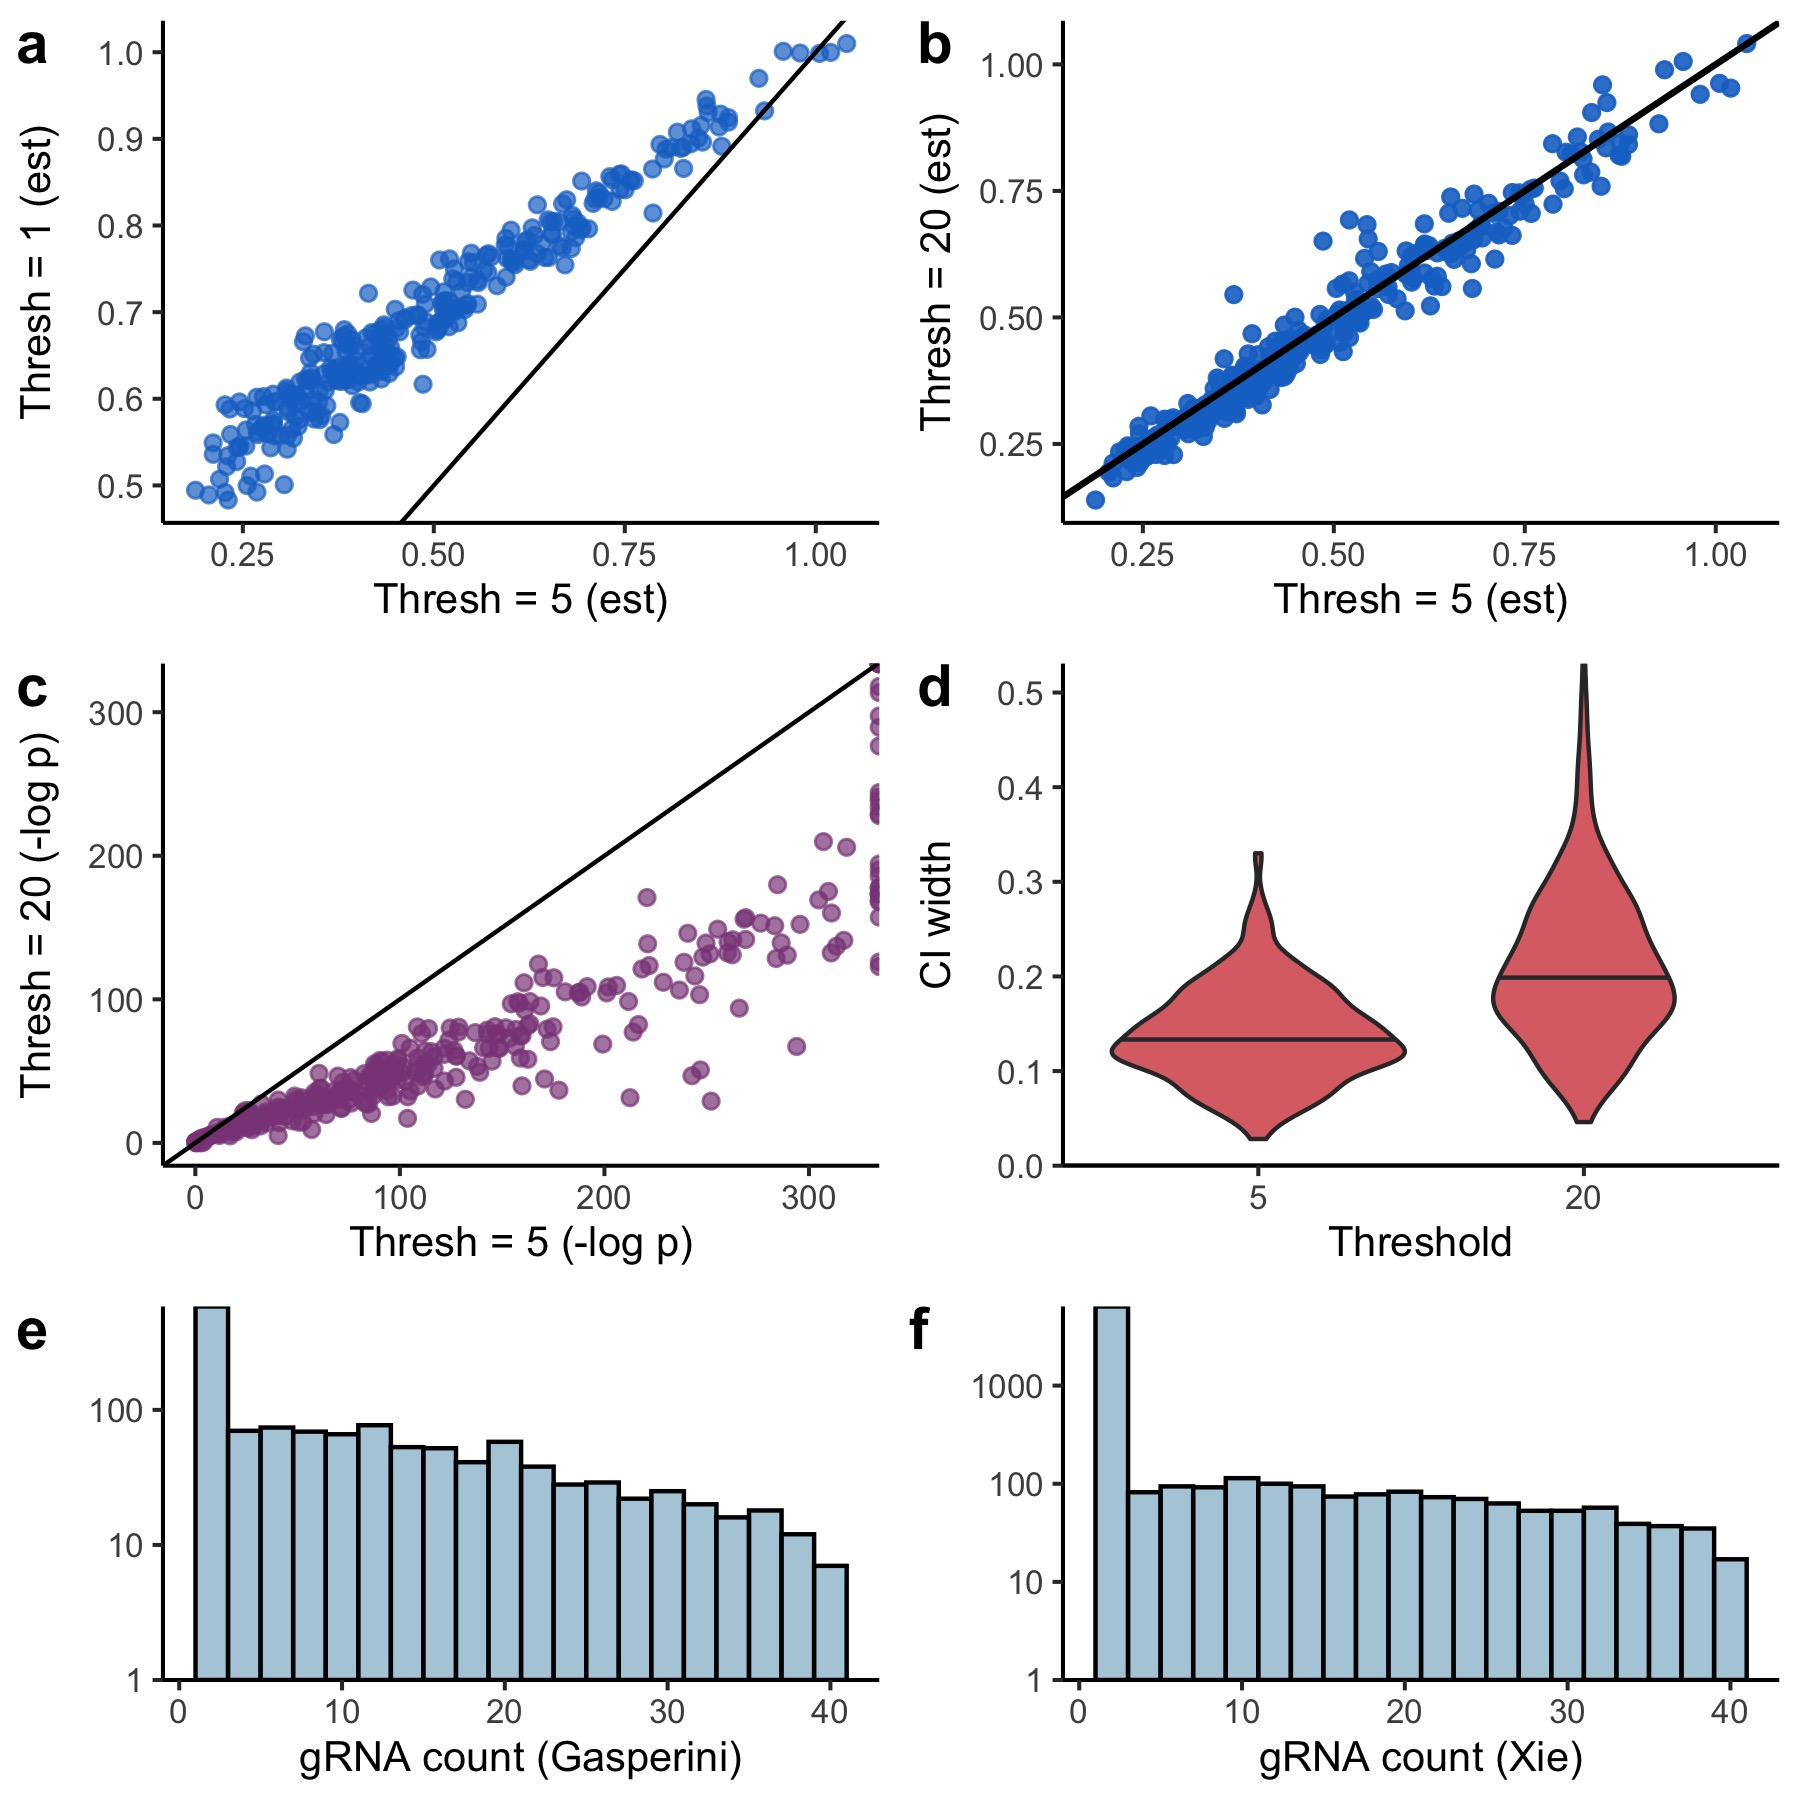
\includegraphics[width=1\linewidth]{../../figures/thresholding_empirical/plot}
	\caption{\textbf{Empirical challenges of thresholded regression.}}
	\label{thresholding_empirical}
\end{figure}
\newpage

\subsection{Theoretical analysis}

We study the thresholding method from a theoretical perspective in an idealized Gaussian setting. Suppose that we observe data $(g_1, m_1), \dots, (g_n, m_n)$ from the following model:

\begin{equation}\label{theoretical_model}
\begin{cases}
m_i = \beta^m_0 + \beta^m_1 p_i + \ep_i \\
g_i = \beta^g_0 + \beta^g_1 p_i + \tau_i \\
p_i \sim \textrm{Bern}(\pi) \\
\ep_i, \tau_i \sim N(0,1) \\
p_i \indep \tau_i \indep \ep_i.
\end{cases}
\end{equation}
For a given threshold $c \in \R$, let $\hat{p}_i = \mathbb{I}(g_i \geq c).$ The thresholding estimator $\hat{\beta}^m_1$ for $\beta^m_1$ is given by $$\hat{\beta}^m_1 = \frac{\sum_{i=1}^n (\hat{p}_i - \overline{\hat{p}}) (m_i - \overline{m})}{\sum_{i=1}^n (\hat{p}_i - \overline{\hat{p}})}.$$ The limit in probability (as $n \to \infty$) of $\hat{\beta}^m_0$ is
\begin{equation}\label{thresh_est_intercepts}
\hat{\beta}^m_1 \xrightarrow{P} \beta^m_1 \left(\frac{ \pi( \omega - \E[ \hat{p}_i ])}{ \E[\hat{p}_i] (1 - \E[\hat{p}_i])}\right),
\end{equation}
where
$$\begin{cases}
\omega = 1 - \Phi\left(c - \beta_1^g - \beta_0^g \right) ,\\ \zeta = 1 - \Phi\left( c - \beta^g_0 \right), \\ \E[\hat{p}_i] = \zeta(1-\pi) + \omega\pi. 
\end{cases}$$
Let $\gamma: \R^4 \to \R$ be defined by
$$ \gamma( \beta^g_0, \beta^g_1, c, \pi ) = \frac{\pi (\omega - \E[\hat{p}_i])}{\E[\hat{p}_i] (1 - \E[\hat{p}_i]) }.$$ We call $\gamma$ the \textit{attenuation function}. Observe that \begin{itemize}
\item[i.] $\gamma$ does not depend on $\beta^m_1$ or $\beta^m_0$, and
\item[ii.] $\hat{\beta}^m_1 \xrightarrow{P} [\gamma(\beta_0^g, \beta_1^g, c, \pi)] \beta^m_1.$
\end{itemize}
Let $b: \R^4 \to \R$ be the asymptotic bias of $\hat{\beta}^m_1$. We can express $b$ in terms of $\gamma$ as $$b\left(\beta^g_0, \beta^g_1, c, \pi \right) = \beta^m_1 - \gamma( \beta_0^g, \beta_1^g, c, \pi) \beta^m_1 = \beta^m_1 \left[ 1- \gamma(\beta^g_0, \beta^g_1, c, \pi) \right].$$ The asymptotic bias vanishes when the attenuation function equals $1$.

\begin{center}
\textbf{Bias as a function of threshold (Panel a)}
\end{center}

To investigate the basic question of ``What is a good threshold selection strategy?'', we study the relationship between the asymptotic bias $b$ of $\hat{\beta}^m_1$ and the selected threshold $c$. For simplicity, we set the perturbation probability $\pi$ to $1/2$. Additionally, without loss of generality, we set the target of inference $\beta^m_1$ to $1$. Let $c_\textrm{bayes} \in \R$ be the Bayes-optimal decision boundary for classifying cells as perturbed or unperturbed, i.e. $$c_\textrm{bayes} = \argmin_{c \in \R} \P(\hat{p}_i \neq p_i).$$ Simple algebra shows that $c_\textrm{bayes} = \beta_0^g + (1/2) \beta^g_1.$ Below, we state several results relating the limiting bias $b$ of $\hat{\beta}^m_1$ to $c_\textrm{bayes}$ and $\beta^g_1$. We defer proofs to the appendix.

\begin{itemize}
\item[1.] The Bayes-optimal threshold $c_\textrm{bayes}$ is a critical value of the bias function $b$ (Figure \ref{thresholding_theoretical}a, all panels), i.e. 
$$ \frac{\partial b( \beta^g_0, \beta^g_1, c, 1/2)}{\partial c} \vline_{c = c_\textrm{bayes}} = 0.$$
\item[2.] For certain values of $\beta^g_0$ and $\beta^g_1$, $c_\textrm{bayes}$ is a maximizer of the bias (Figure \ref{thresholding_theoretical}a, left); for other values of $\beta^g_0$ and $\beta^g_1$, $c_\textrm{bayes}$ is a minimizer of the bias (Figure \ref{thresholding_theoretical}a, right).
\item[3.] The limit of the bias in $c$ is $1/2$, i.e. 
$$\lim_{c \to \infty} b(\beta^g_0, \beta^g_1, c, 1/2) = 1/2.$$ In other words, we always can set the threshold to a large number and achieve a bias of $1/2$ (Figure \ref{thresholding_theoretical}a, all panels). This fact establishes an upper bound on the bias of thresholded regression (under optimal threshold selection).
\item[4.] For $\beta^g_1 < 2 \Phi(3/4) \approx 1.35$, $c = c_\textrm{bayes}$ yields a \textit{larger} bias than $c = \infty$ (Figure \ref{thresholding_theoretical}a, left); for $\beta^g_1 > 2 \Phi(3/4)$, $c_\textrm{bayes}$ yields a \textit{smaller} bias than $c = \infty$ (Figure \ref{thresholding_theoretical}a, right); finally, for $\beta^g_1 = 2 \Phi(3/4)$, $c = c_\textrm{bayes}$ and $c = \infty$ both yield a bias of $1/2$ (Figure \ref{thresholding_theoretical}a, middle).
\item[5.] The bias decreases monotonically as $\beta_1^g$ increases (Figure \ref{thresholding_theoretical}a; fix threshold and scan panels from left to right). This is consistent with the intuition that the problem becomes easier as the gRNA mixture distribution becomes increasingly well-separated.
\item[6.] For all $\beta^g_0, \beta^g_1,$ and $c \in \R,$ the bias is strictly greater than $0$ and less than $2$ (Figure \ref{thresholding_theoretical}a, all panels). Therefore, the thresholding method suffers from attenuation bias.% a common phenomenon in errors-in-variables models.
\end{itemize}

These results are subtle, but we can summarize them as follows. First, selecting a threshold that minimizes the bias is deceptively challenging, as there is no rule of thumb that we can apply universally (e.g., ``always choose the Bayes-optimal decision boundary'' or ``always choose a large number''). Second, even if we \textit{have} selected a good threshold, the thresholding method incurs a strict attenuation bias.

\begin{center}
\textbf{Generalizing to $\pi \in [0,1/2]$ (Panel b)}
\end{center}

Next, we generalize the expression for bias when the threshold is large to arbitrary $\pi \in [0,1/2]$. The following simple relationship holds:
$$ \lim_{ c \to \infty } b(\beta^g_0, \beta^g_1, c, \pi) = \pi.$$ In other words, when the perturbation probability is equal to $\pi$, setting the threshold to a large number yields a bias of $\pi$ (Figure \ref{thresholding_theoretical}b). We can build intuition for this result by considering an extreme example. When $\pi$ is very small (e.g., $\pi = 0.01$), almost all cells are unperturbed. Therefore, in selecting a large threshold, one correctly classifies nearly all unperturbed cells as unperturbed; on the other hand, the \textit{perturbed} cells that one misclassifies as \textit{unperturbed} are swamped in number by the truly unperturbed cells, resulting in a small bias.

\begin{figure}[h!]
	\centering
	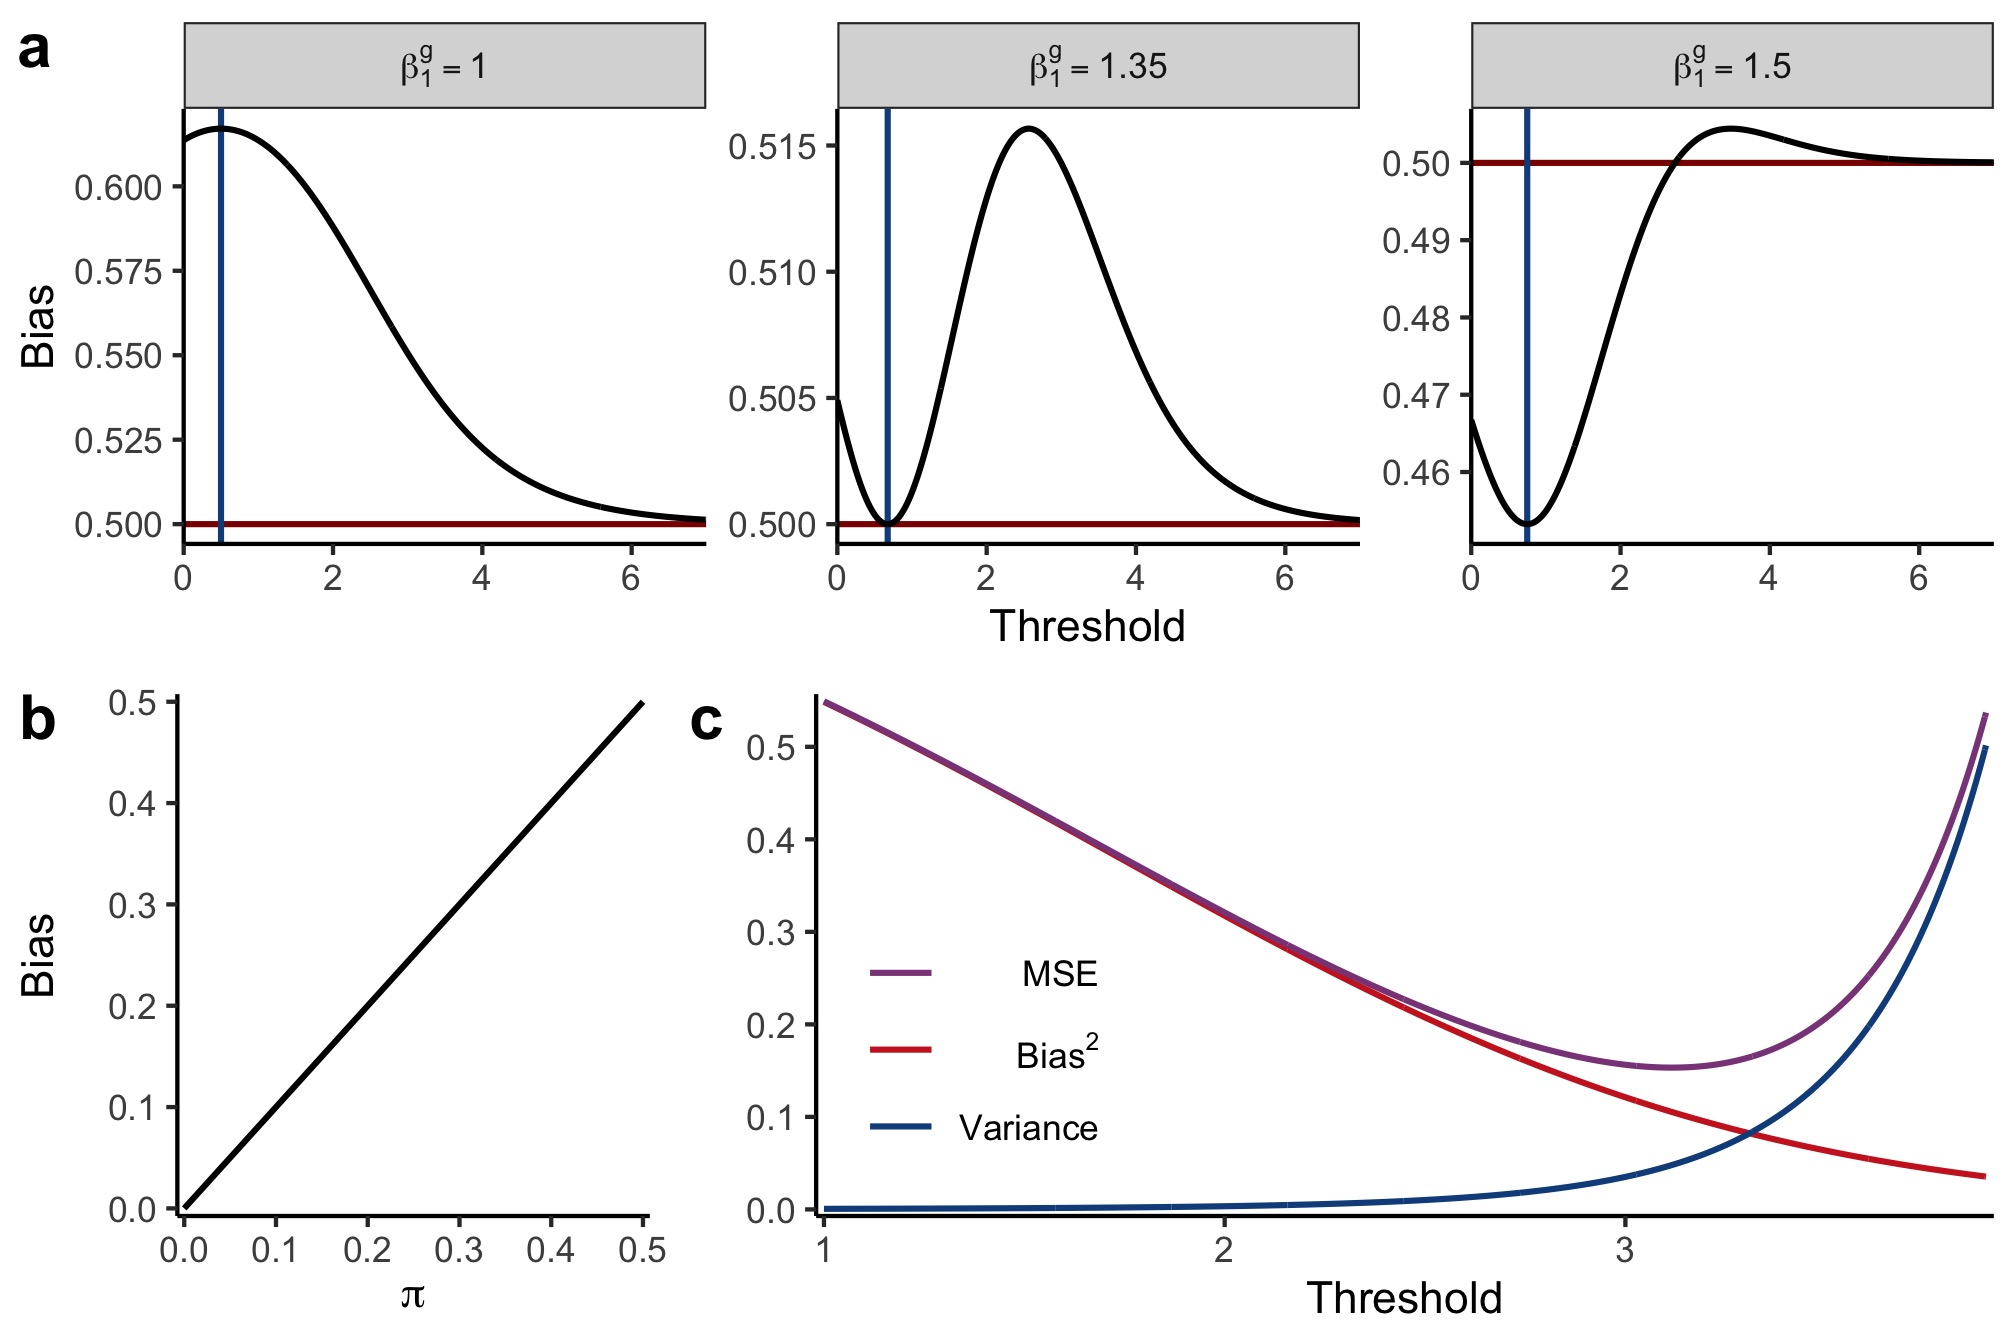
\includegraphics[width=1\linewidth]{../../figures/thresholding_theoretical/plot}
	\caption{\textbf{Theoretical challenges of thresholded regression.}}
	\label{thresholding_theoretical}
\end{figure}

\begin{center}
	\textbf{Bias-variance tradeoff (Panel c)}
\end{center}

Finally, to shed light on limitations of the large threshold selection strategy, we study the variance of the thresholding estimator. Let $v$ denote the limiting variance of scaled estimator $\sqrt{n} \hat{\beta}^m_1$, i.e.,
$$v(\beta^g_0, \beta^g_1, c, \pi) = \lim_{n \to \infty} \V(\sqrt{n} \hat{\beta}^m_1).$$ The limiting variance of $\sqrt{n} \hat{\beta}^m_1$ grows without bound as the threshold $c$ tends to infinity: 
$$ \lim_{c \to \infty} v(\beta^g_0, \beta^g_1, c, \pi) = \infty.$$ Thus, while selecting a large threshold is effective from a bias reduction standpoint when $\pi$ is small, it causes the variance to explode.

To more precisely characterize the bias-variance tradeoff of the thresholding method, we consider a slightly simpler model: we set $\beta^m_0$ and $\beta^g_0$ to zero in (\ref{theoretical_model}) and study the no-intercept least squares estimator
$$ \hat{\beta}^m_1 =  \frac{ \sum_{i=1}^n \hat{p}_i m_i }{ \sum_{i=1}^n \hat{p}_i^2}.$$ We uncover an exact bias-variance tradeoff as a function of the selected threshold (Figure \ref{thresholding_theoretical}c). The bias-variance analysis reveals that the best strategy for minimizing mean-squared error is to select a threshold that induces moderate bias. (A downside of this approach, of course, is that constructing valid confidence intervals becomes more challenging.)


% These difficulties motivate our core research question: does bypassing thresholding altogether lead to better estimation and inference in single-cell CRISPR screens? To answer this question, we propose GLM-EIV, method for single-cell CRISPR screen analysis that models gRNA counts directly.

\section{GLM-EIV}

\section{Simulation studies}

\section{Real data analysis}

\section{Discussion}

\section{Appendix}

\subsection{Theoretical details for thresholding estimator}

This section contains proofs for results presented the section ``Theoretical analysis of thresholding estimator.'' 

\subsubsection{Limit of $\hat{\beta}^m_1$ in Gaussian model with intercepts}

Consider the thresholding estimator $\hat{\beta}^m_1$ for the Gaussian model with intercepts (\ref{theoretical_model}). Dividing by $n$ in (\ref{thresh_est_intercepts}), we can express $\hat{\beta}^m_1$ as
$$ \hat{\beta}^m_1 = \frac{ \frac{1}{n} \sum_{i=1}^n ( \hat{p}_i - \overline{\hat{p}_i})(m_i - \overline{m})}{ \frac{1}{n} \sum_{i=1}^n (\hat{p}_i - \overline{\hat{p}})}.$$ By weak LLN,
$$ \hat{\beta}^m_1 \xrightarrow{P} \frac{\textrm{Cov}(\hat{p}_i, m_i)}{\V\left(\hat{p}_i\right)}.$$ To compute this quantity, we first compute several simpler quantities:
\begin{itemize}
\item[1.] Expectation of $m_i$: $\E[m_i] = \beta^m_0 + \beta^m_1\pi.$
\item[2.] Expectation of $\hat{p}_i$: Let $f$ denote the $N(0,1)$ density. Then \begin{multline*}
\E[\hat{p}_i] = \P\left[\hat{p}_i = 1\right] = \P\left[\beta^g_0 + \beta^g_1 + \tau_i \geq c \right] = \\ \textrm{(By LOTP) } \P\left[ \beta^g_0 + \tau_i \geq c \right]\P\left[p_i = 0\right] + \P\left[ \beta^g_0 + \beta^g_1 + \tau_i \geq c \right] \P[p_i = 1] \\ = \P\left[ \tau_i \geq c - \beta^g_0\right](1- \pi) + \P\left[ \tau_i \geq c - \beta^g_1 - \beta^g_0 \right](\pi) \\ = \left(\int_{c - \beta^g_0}^\infty f\right) (1 - \pi) + \left( \int_{c - \beta^g_1 - \beta^g_0}^\infty f \right)(\pi) = \zeta(1-\pi) + \omega \pi,
\end{multline*}
where $$\zeta = \int_{c - \beta_0^g}^\infty f = 1 - \Phi(c - \beta^g_0)$$ and 
$$ \omega = \int_{c - \beta^g_1 - \beta^g_0}^\infty f = 1 - \Phi(c - \beta^g_1 - \beta^g_0).$$
\item[3.] Expectation of $\hat{p}_i p_i$: 
$$\E\left[ \hat{p}_i p_i \right] = \E\left[ \hat{p}_i | p_i = 1 \right] \P\left[ p_i =1 \right] = \P\left[ \beta^g_0 + \beta^g_1 + \tau_i \geq c \right] \pi = \omega \pi.$$
\item[4.] Expectation of $\hat{p}_i m_i$:
\begin{multline*}
\E\left[\hat{p}_i m_i\right] = \E[\hat{p}_i (\beta^m_0 + \beta^m_1 p_i + \ep_i)] = \beta^m_0 \E\left[\hat{p}_i\right] + \beta^m_1 \E\left[\hat{p}_i p_i\right] + \E[\hat{p}_i \ep_i] \\ = \beta^m_0 \E[\hat{p}_i] + \beta^m_1 \omega \pi + \E[\hat{p}_i] \E[\ep_i] = \beta^m_0 \E[\hat{p}_i] + \beta^m_1 \omega \pi.
\end{multline*}
\item[5.] Variance of $\hat{p}_i$: Because $\hat{p}_i$ is binary, we have that $\V[\hat{p}_i] = \E[\hat{p}_i]\left(1 - \E[\hat{p}_i]\right) .$
\item[6.] Covariance of $\hat{p}_i, m_i$:
\begin{multline*}
\textrm{Cov}\left(\hat{p}_i, m_i\right) = \E\left[\hat{p}_i m_i\right] - \E[\hat{p}_i] \E[m_i] = \beta^m_0 \E[\hat{p}_i] + \beta^m_1 \omega \pi - \E[\hat{p}_i]( \beta^m_0 + \beta^m_1 \pi)\\ = \beta^m_1 \omega \pi - \E[\hat{p}_i] \beta_1^m \pi = \beta^m_1 \pi \left( \omega - \E[\hat{p}_i]\right).
\end{multline*}
Combining these expressions, we have that
$$ \hat{\beta}^m_1 \xrightarrow{P} \frac{\beta^m_1 \pi (\omega - \E[\hat{p}_i])}{\E[\hat{p}_i](1 - \E[\hat{p}_i])} = \beta^m_1 \gamma(\beta^g_0, \beta^g_1, c, \pi).$$
\end{itemize}
\subsubsection{Re-expressing $\gamma$ when $\pi = 1/2$}

Suppose $\pi = 1/2$. We rewrite the attenuation fraction $\gamma$ in a way that makes it more amenable to theoretical analysis. We leverage the fact that $f$ integrates to unity and is even. First,
\begin{multline*} \E\left[\hat{p}_i\right] = (1/2) \left( \int_{c - \beta^g_0}^\infty f \right) + (1/2) \left( \int_{c - \beta_0^g - \beta_1^g}^\infty f \right) \\ = (1/2) \left( \int_{-\infty}^{ \beta_0^g - c} f \right) + (1/2) \left( \int_{-\infty}^{ \beta^g_0 + \beta^g_1 - c} f \right). \end{multline*} and so \begin{multline*} 1 - \E\left[\hat{p}_i\right] = (1/2) + (1/2) - \E[\hat{p}_i]  = (1/2) \left(1 - \int_{c - \beta_0^g}^\infty f \right)  + (1/2) \left( 1 - \int_{c - \beta^g_0 - \beta^g_1}^\infty f \right) \\ = (1/2) \left( \int_{-\infty}^{c - \beta^g_0} f \right) + (1/2) \left( \int_{-\infty}^{c - \beta_0^g - \beta_1^g} f \right)
\end{multline*}
Next,
$$\omega = \int_{c - \beta^g_1 - \beta^g_0}^\infty f,$$ and so
\begin{multline*}
\omega - \E[\hat{p}_i]  = \left( \int_{c - \beta^g_1 - \beta^g_0}^\infty f \right) - (1/2) \left( \int_{c - \beta^g_0}^\infty f \right) - (1/2) \left( \int_{c - \beta_0^g - \beta_1^g}^\infty f \right) \\ = (1/2) \left(\int_{c - \beta^g_0 - \beta^g_1 }^\infty f \right) - (1/2) \left(\int_{c - \beta^g_0}^\infty f \right) =  (1/2)\left(\int_{-\infty}^{\beta_0^g + \beta_1^g - c} f \right) - (1/2) \left( \int_{-\infty}^{ \beta_0^g - c} f \right).
\end{multline*}
Therefore,
\begin{multline*}
\gamma(\beta_0^g, \beta_1^g, c, 1/2) = \frac{ (1/2) (\omega - \E[\hat{p}_i])}{ \E[\hat{p}_i] \left(1 - \E[\hat{p}_i] \right)} \\ = \frac{(1/2) \left[ (1/2) \left( \int_{ -\infty}^{\beta_0^g + \beta_1^g - c} f \right) - (1/2) \left( \int_{-\infty}^{ \beta_0^g - c} f \right) \right]}{ \left[(1/2) \left( \int_{-\infty}^{ \beta_0^g - c} f \right) + (1/2) \left( \int_{-\infty}^{ \beta^g_0 + \beta^g_1 - c} f \right) \right] \left[ (1/2) \left( \int_{-\infty}^{c - \beta^g_0} f \right) + (1/2) \left( \int_{-\infty}^{c - \beta_0^g - \beta_1^g} f \right) \right]} \\ = \frac{\left( \int_{ -\infty}^{\beta_0^g + \beta_1^g - c} f \right) - \left( \int_{-\infty}^{ \beta_0^g - c} f \right) }{ \left[ \left( \int_{-\infty}^{ \beta_0^g - c} f \right) + \left( \int_{-\infty}^{ \beta^g_0 + \beta^g_1 - c} f \right) \right] \left[\left( \int_{-\infty}^{c - \beta^g_0} f \right) + \left(\int_{-\infty}^{c - \beta_0^g - \beta_1^g} f \right) \right]}.
\end{multline*}
Treating $\beta^g_0$ as a fixed constant, define 
$$g(\beta^g_1, c) = \left( \int_{ -\infty}^{\beta_0^g + \beta_1^g - c} f \right) - \left( \int_{-\infty}^{ \beta_0^g - c} f \right) ,$$ and
$$h(\beta^g_1, c) = \left[ \left( \int_{-\infty}^{ \beta_0^g - c} f \right) + \left( \int_{-\infty}^{ \beta^g_0 + \beta^g_1 - c} f \right) \right] \left[\left( \int_{-\infty}^{c - \beta^g_0} f \right) + \left(\int_{-\infty}^{c - \beta_0^g - \beta_1^g} f \right) \right].$$ We can write
$$\gamma(\beta^g_0, \beta^g_1, c, 1/2) = \frac{ g(\beta^g_1, c) }{ h(\beta^g_1, c)}.$$ We will write $g(\beta^g_1, \cdot)$ (resp., $g(\cdot, \beta^g_1)$) to denote the univariate function that results from holding the second (resp., first) argument of $g$ fixed. We adopt similar notation for $h$. 

\subsubsection{Bayes-optimal decision boundary as a critical value}
Let $c_\textrm{bayes} = \beta^g_0 + (1/2)\beta^g_1.$ We show that $c = c_\textrm{bayes}$ is a critical value of $\gamma$ for $\pi = 1/2$ and fixed $(\beta^g_0, \beta^g_1)$ , i.e, $$\frac{\partial  \gamma(\beta^g_0, \beta^g_1, c, 1/2)}{ \partial c} \vline_{[c = c_\textrm{bayes}]} = 0.$$ By quotient rule,
$$ \frac{\partial  \gamma(\beta^g_0, \beta^g_1, c, 1/2)}{ \partial c} = \frac{g'(\cdot, c) h(\cdot, c) - g(\cdot, c) h'(\cdot, c)}{\left[ h(\cdot, c) \right]^2}.$$ First,
$$g'(\cdot, c) = - f( \beta^g_0 + \beta^g_1 - c ) + f(\beta^g_0 - c).$$ Second, 
\begin{multline*}
h'(\cdot, c) = -[f(\beta^g_0 - c)  + f( \beta^g_0 + \beta^g_1 - c )]  \left[\left( \int_{-\infty}^{c - \beta^g_0} f \right) + \left(\int_{-\infty}^{c - \beta_0^g - \beta_1^g} f \right) \right] \\ +[ f(c - \beta^g_0) + f(c - \beta^g_0 - \beta^g_1) ] \left[ \left( \int_{-\infty}^{ \beta_0^g - c} f \right) + \left( \int_{-\infty}^{ \beta^g_0 + \beta^g_1 - c} f \right) \right].
\end{multline*}
Evaluating $g'(\cdot, c)$ and $h'(\cdot, c)$ at $c = c_\textrm{bayes} $, we find that
$$g'(\beta^g_0 + (1/2) \beta^g_1) = -f(\beta^g_1/2) + f(- \beta^g_1/2) = -f(\beta^g_1/2) + f(\beta^g_1/2) = 0,$$ where the second equality follows from the evenness of $f$. Similarly, 
\begin{multline*}
 h'(\beta^g_0 + (1/2) \beta^g_1) = - \left[ f( -\beta^g_1/2) + f( \beta^g_1/2 ) \right] \left[ \int_{-\infty}^{ \beta^g_1/2} f + \int_{-\infty}^{ -\beta^g_1/2} f \right] + \\ \left[ f( \beta^g_1/2) + f( -\beta^g_1/2 ) \right] \left[ \int_{-\infty}^{ -\beta^g_1/2} f + \int_{-\infty}^{ \beta^g_1/2 f} \right] = 0.
\end{multline*}
We conclude that
$$ \frac{\partial \gamma(\beta^g_0, \beta^g_1, c, 1/2)}{ \partial c} \vline_{[c = c_\textrm{bayes}]} = \frac{0\cdot h(\cdot, c_\textrm{bayes}) - g(\cdot, c_\textrm{bayes}) \cdot 0}{ h(\cdot, c_\textrm{bayes})^2} = 0.$$ Finally, because asymptotic bias $b$ can be expressed in terms of $\gamma$ as $$b(\beta^g_0. \beta^g_1, c, \pi) = \beta^m_1 \left[ 1 - \gamma(\beta^g_0, \beta^g_1, c, \pi) \right],$$ it follows that $c = c_\textrm{bayes}$ is a critical value of $b$ for $\pi = 1/2$ and fixed $(\beta^g_0, \beta^g_1)$.

\subsubsection{Limit in $\beta^g_1$}

We compute the limit of $\gamma(\beta^g_0, \beta^g_1, c, 1/2)$ in $\beta^g_1.$ We have that

\begin{multline*}
 \lim_{\beta^g_1 \to \infty } \gamma(\beta^g_0, \beta^g_1, c, 1/2) = \frac{ 1 - \int_{-\infty}^{\beta^g_0 - c } f}{\left[ 1 + \int_{-\infty}^{ \beta^g_0 - c} f \right] \left[\int_{-\infty}^{ c - \beta^g_0} f \right]} \\ = \frac{\int_{-\infty}^{c - \beta^g_0} f }{ \left[1 + \int_{-\infty}^{ \beta^g_0 - c} f \right] \left[\int_{-\infty}^{ c - \beta^g_0} f \right]} = \frac{1}{1 + \int_{-\infty}^{\beta^g_0 - c} f} < 1.
 \end{multline*}
 
 Similarly,
\begin{multline*}
\lim_{\beta^g_1 \to -\infty} \gamma(\beta^g_0, \beta^g_1, c, 1/2) = \frac{ -\int_{-\infty}^{\beta^g_0 - c} f }{\left[ \int_{-\infty}^{\beta^g_0 - c} f \right] \left[ \int_{-\infty}^{c - \beta^g_0} f + 1 \right]} = \frac{-1}{1 + \int_{-\infty}^{c - \beta^g_0} f} > -1.
\end{multline*}

\subsubsection{Monotonicity in $\beta^g_1$}

\subsection{Derivation of EM algorithm}

\subsection{Derivation of observed information matrix}

\subsection{Implementation using R family objects}

\subsection{Statistical accelerations to GLM-EIV}

\subsection{Additional simulation results}


\bibliographystyle{unsrt}
\newpage
\bibliography{/Users/timbarry/optionFiles/glmeiv.bib}


\end{document}
